\documentclass[12pt,a4paper,twoside,openright]{report}
\let\openright=\cleardoublepage



%%% Choose a language %%%

\newif\ifEN
\ENtrue   % uncomment this for english
%\ENfalse   % uncomment this for czech

%%% Configuration of the title page %%%

\def\ThesisTitleStyle{mff} % MFF style
%\def\ThesisTitleStyle{cuni} % uncomment for old-style with cuni.cz logo
%\def\ThesisTitleStyle{natur} % uncomment for nature faculty logo

\def\UKFaculty{Faculty of Mathematics and Physics}
%\def\UKFaculty{Faculty of Science}

\def\UKName{Charles University in Prague} % this is not used in the "mff" style

% Thesis type names, as used in several places in the title
\def\ThesisTypeTitle{\ifEN BACHELOR THESIS \else BAKALÁŘSKÁ PRÁCE \fi}
%\def\ThesisTypeTitle{\ifEN MASTER THESIS \else DIPLOMOVÁ PRÁCE \fi}
%\def\ThesisTypeTitle{\ifEN RIGOROUS THESIS \else RIGORÓZNÍ PRÁCE \fi}
%\def\ThesisTypeTitle{\ifEN DOCTORAL THESIS \else DISERTAČNÍ PRÁCE \fi}
\def\ThesisGenitive{\ifEN bachelor \else bakalářské \fi}
%\def\ThesisGenitive{\ifEN master \else diplomové \fi}
%\def\ThesisGenitive{\ifEN rigorous \else rigorózní \fi}
%\def\ThesisGenitive{\ifEN doctoral \else disertační \fi}
\def\ThesisAccusative{\ifEN bachelor \else bakalářskou \fi}
%\def\ThesisAccusative{\ifEN master \else diplomovou \fi}
%\def\ThesisAccusative{\ifEN rigorous \else rigorózní \fi}
%\def\ThesisAccusative{\ifEN doctoral \else disertační \fi}



%%% Fill in your details %%%

% (Note: \xxx is a "ToDo label" which makes the unfilled visible. Remove it.)
\def\ThesisTitle{Implicit Information Extraction from News Stories}
\def\ThesisAuthor{Hynek Kydlíček}
\def\YearSubmitted{2023}

% department assigned to the thesis
\def\Department{Institute of Formal and Applied Linguistics}
% Is it a department (katedra), or an institute (ústav)?
\def\DeptType{Institute}

\def\Supervisor{Mgr. Jindřich Libovický, Ph.D.}
\def\SupervisorsDepartment{Institute of Formal and Applied Linguistics}

% Study programme and specialization
\def\StudyProgramme{Computer Science}
\def\StudyBranch{Artificial Intelligence Bc.}

\def\Dedication{%
I would like to thank my supervisor Mgr. Jindřich Libovický, Ph.D. for his guidance and support throughout the whole process.
I would also like to thank my family and friends for their support and encouragement.
}

\def\AbstractEN{%
This work deals with information extraction from Czech News Stories. We focus on 4 tasks:
Publishing server, Article's category, Author's textual gender and Publication day of week. 
As no dataset for these tasks exists, this work presents a new extensive dataset of 1.5M Czech news articles
with various metadata. With the dataset, we also publish a new tool C'monCrawl for extracting resources from CommonCrawl
archive. Tasks are then solved using various machine learning methods mainly based on Transformer architecture.
Our work sets strong baseline results on the said dataset allowing for further research in the field.
}

\def\AbstractCS{%
Tato práce se zabývá extrakcí informací z českých zpravodajských článků. Zaměřujeme se na 4 úlohy:
Vydavatelský server, kategorie článku, textový gender autra a den vydání.
Protože pro tyto úlohy neexistuje žádná datová sada, představuje tato práce novou rozsáhlou datovout sadu
čítající 1,5 milionu českých zpravodajských článků s rozličnými metadaty.
Spolu s datovou sadou publikujeme také nový nástroj C'monCrawl pro extrakci zdrojů z CommonCrawl archivu.
archivu. Úlohy jsou pak řešeny pomocí různých metod strojového učení založených především na architektuře Transformer.
Naše práce představuje silný základný výsledek na uvedené datové sadě, který umožňuje další výzkum v této oblasti.
}

% 3 to 5 keywords (recommended), each enclosed in curly braces.
% Keywords are useful for indexing and searching for the theses by topic.
\def\Keywords{%
{Information Extraction}, {Server}, {Category}, {Gender} 
{Day Of Week}, {C'monCrawl}, {Czech News Dataset}
}

% If your abstracts are long and do not fit in the infopage, you can make the
% fonts a bit smaller by this setting. (Also, you should try to compress your abstract more.)
% Alternatively, consider increasing the size of the page by uncommenting the
% geometry modification in thesis.tex.
\def\InfoPageFont{}
%\def\InfoPageFont{\small}  %uncomment to decrease font size

\ifEN\relax\else
% If you are writing a czech thesis, you additionally need to fill in the
% english translation of the metadata here!
\def\ThesisTitleEN{\xxx{Thesis title in English}}
\def\DepartmentEN{\xxx{Name of the department in English}}
\def\DeptTypeEN{\xxx{Department}}
\def\SupervisorsDepartmentEN{\xxx{Superdepartment}}
\def\StudyProgrammeEN{\xxx{study programme}}
\def\StudyBranchEN{\xxx{study branch}}
\def\KeywordsEN{%
\xxx{{key} {words}}
}
\fi


\usepackage[a-2u]{pdfx}

\ifEN\else\usepackage[czech,shorthands=off]{babel}\fi
\usepackage[utf8]{inputenc}
\usepackage[T1]{fontenc}

% See https://en.wikipedia.org/wiki/Canons_of_page_construction before
% modifying the size of printable area. LaTeX defaults are great.
% If you feel it would help anything, you can enlarge the printable area a bit:
%\usepackage[textwidth=390pt,textheight=630pt]{geometry}
% The official recommendation expands the area quite a bit (looks pretty harsh):
%\usepackage[textwidth=145mm,textheight=247mm]{geometry}

%%% FONTS %%%
\usepackage{lmodern} % TeX "original" (this sets up the latin mono)

% Optionally choose an override for the main font for typesetting
\usepackage[mono=false]{libertinus} % popular for comp-sci (ACM uses this)
%\usepackage{tgschola} % Schoolbook-like (gives a bit of historic feel)
%\usepackage[scale=0.96]{tgpagella} % Palladio-like (popular in formal logic).

% Optionally choose a custom sans-serif fonts (e.g. for figures and tables).
% Default sans-serif font is usually Latin Modern Sans. Some font packages
% (e.g. libertinus) replace that with a better matching sans-serif font.
%\usepackage{tgheros} % recommended and very readable (Helvetica-like)
%\usepackage{FiraSans} % looks great
% DO NOT typeset the main text in sans-serif font!
% The serifs make the text easily readable on the paper.

% IMPORTANT FONT NOTE: Some fonts require additional PDF/A conversion using
% the pdfa.sh script. These currently include only 'tgpagella'; but various
% other fonts from the texlive distribution need that too (mainly the Droid
% font family).


% some useful packages
\usepackage{microtype}
\usepackage{amsmath,amsfonts,amsthm,bm}
\usepackage{graphicx}
\usepackage{xcolor}
\usepackage{booktabs}
\usepackage{caption}
\usepackage{floatrow}

% load bibliography tools
\usepackage[backend=bibtex,natbib,style=numeric,sorting=none]{biblatex}
% alternative with alphanumeric citations (more informative than numbers):
% \usepackage[backend=bibtex,natbib,style=alphabetic]{biblatex}
% \usepackage[]{biblatex}
%
% alternatives that conform to iso690
% (iso690 is not formally required on MFF, but may help elsewhere):
%\usepackage[backend=bibtex,natbib,style=iso-numeric,sorting=none]{biblatex}
%\usepackage[backend=bibtex,natbib,style=iso-alphabetic]{biblatex}
%
% additional option choices:
%  - add `giveninits=true` to typeset "E. A. Poe" instead of full Edgar Allan
%  - `terseinits=true` additionaly shortens it to nature-like "Poe EA"
%  - add `maxnames=10` to limit (or loosen) the maximum number of authors in
%    bibliography entry before shortening to `et al.` (useful when referring to
%    book collections that may have hundreds of authors)
%  - for additional flexibility (e.g. multiple reference sections, etc.),
%    remove `backend=bibtex` and compile with `biber` instead of `bibtex` (see
%    Makefile)
%  - `sorting=none` causes the bibliography list to be ordered by the order of
%    citation as they appear in the text, which is usually the desired behavior
%    with numeric citations. Additionally you can use a style like
%    `numeric-comp` that compresses the long lists of citations such as
%    [1,2,3,4,5,6,7,8] to simpler [1--8]. This is especially useful if you plan
%    to add tremendous amounts of citations, as usual in life sciences and
%    bioinformatics.
%  - if you don't like the "In:" appearing in the bibliography, use the
%    extended style (`ext-numeric` or `ext-alphabetic`), and add option
%    `articlein=false`.
%
% possibly reverse the names of the authors with the default styles:
%\DeclareNameAlias{default}{family-given}

% load the file with bibliography entries
\addbibresource{refs.bib}

% remove this if you won't use fancy verbatim environments
\usepackage{fancyvrb}

% remove this if you won't typeset TikZ graphics
\usepackage{tikz}
\usetikzlibrary{positioning} %add libraries as needed (shapes, decorations, ...)

% remove this if you won't typeset any pseudocode
\usepackage{algpseudocode}
\usepackage{algorithm}

% remove this if you won't list any source code
\usepackage{listings}


\hypersetup{unicode}
\hypersetup{breaklinks=true}

\usepackage[noabbrev]{cleveref}


% various forms of TODOs (you should remove this before submitting)
\usepackage[textsize=tiny, backgroundcolor=yellow!25, linecolor=black!25]{todonotes}
\newcommand{\xxx}[1]{\textcolor{red!}{#1}}

 % remove this before compiling the final version


% use this for typesetting a chapter without a number, e.g. intro and outro
\def\chapwithtoc#1{
\chapter*{#1}
\addcontentsline{toc}{chapter}{#1}
}

% If there is a line/figure overflowing into page margin, this will make the
% problem evident by drawing a thick black line at the overflowing spot. You
% should not disable this.
\overfullrule=3mm

% The maximum stretching of a space. Increasing this makes the text a bit more
% sloppy, but may prevent the overflows by moving words to next line.
\emergencystretch=1em

\ifEN
\theoremstyle{plain}
\newtheorem{thm}{Theorem}
\newtheorem{lemma}[thm]{Lemma}
\newtheorem{claim}[thm]{Claim}
\newtheorem{defn}{Definition}
\theoremstyle{remark}
\newtheorem*{cor}{Corollary}
\else
\theoremstyle{plain}
\newtheorem{thm}{Věta}
\newtheorem{lemma}{Lemma}
\newtheorem{claim}{Tvrzení}
\newtheorem{defn}{Definice}
\theoremstyle{remark}
\newtheorem*{cor}{Důsledek}
\fi

\newenvironment{myproof}{
  \par\medskip\noindent
  \textit{\ifEN Proof \else Důkaz \fi}.
}{
\newline
\rightline{$\qedsymbol$}
}

% real/natural numbers
\newcommand{\R}{\mathbb{R}}
\newcommand{\N}{\mathbb{N}}

% asymptotic complexity
\newcommand{\asy}[1]{\mathcal{O}(#1)}

% listings and default lstlisting config (remove if unused)
\DeclareNewFloatType{listing}{}
\floatsetup[listing]{style=ruled}

\DeclareCaptionStyle{thesis}{style=base,font={small,sf},labelfont=bf,labelsep=quad}
\captionsetup{style=thesis}
\captionsetup[algorithm]{style=thesis,singlelinecheck=off}
\captionsetup[listing]{style=thesis,singlelinecheck=off}

% Uncomment for table captions on top. This is sometimes recommended by the
% style guide, and even required for some publication types.
%\floatsetup[table]{capposition=top}
%
% (Opinionated rant:) Captions on top are not "compatible" with the general
% guideline that the tables should be formatted to be quickly visually
% comprehensible and *beautiful* in general (like figures), and that the table
% "head" row (with column names) should alone communicate most of the content
% and interpretation of the table. If you just need to show a long boring list
% of numbers (because you have to), either put some effort into showing the
% data in an attractive figure-table, or move the data to an attachment and
% refer to it, so that the boredom does not impact the main text flow.
%
% You can make the top-captions look much less ugly by aligning the widths of
% the caption and the table, with setting `framefit=yes`, as shown below.  This
% additionally requires some extra markup in your {table} environments; see the
% comments in the example table in `ch2.tex` for details.
%\floatsetup[table]{capposition=top,framefit=yes}

\ifEN\floatname{listing}{Listing}
\else\floatname{listing}{Výpis kódu}\fi
\lstset{ % use this to define styling for any other language
  language=C++,
  tabsize=2,
  showstringspaces=false,
  basicstyle=\footnotesize\tt\color{black!75},
  identifierstyle=\bfseries\color{black},
  commentstyle=\color{green!50!black},
  stringstyle=\color{red!50!black},
  keywordstyle=\color{blue!75!black}}

% Czech versions of the used cleveref references (It's not as convenient as in
% English because of declension, cleveref is limited to sg/pl nominative. Use
% plain \ref to dodge that.)
\ifEN\relax\else
\crefname{chapter}{kapitola}{kapitoly}
\Crefname{chapter}{Kapitola}{Kapitoly}
\crefname{section}{sekce}{sekce}
\Crefname{section}{Sekce}{Sekce}
\crefname{subsection}{sekce}{sekce}
\Crefname{subsection}{Sekce}{Sekce}
\crefname{subsubsection}{sekce}{sekce}
\Crefname{subsubsection}{Sekce}{Sekce}
\crefname{figure}{obrázek}{obrázky}
\Crefname{figure}{Obrázek}{Obrázky}
\crefname{table}{tabulka}{tabulky}
\Crefname{table}{Tabulka}{Tabulky}
\crefname{listing}{výpis}{výpisy}
\Crefname{listing}{Výpis}{Výpisy}
\floatname{algorithm}{Algoritmus}
\crefname{algorithm}{algoritmus}{algoritmy}
\Crefname{algorithm}{Algoritmus}{Algoritmy}
\newcommand{\crefpairconjunction}{ a~}
\newcommand{\crefrangeconjunction}{ a~}
\fi
 % use this file for various custom definitions


\begin{document}

% the layout is mandatory, edit only in dire circumstances

\pagestyle{empty}
\hypersetup{pageanchor=false}
\begin{center}

% top part of the layout, this actually differs between faculties

\def\ThesisTitleXmff{%
  \ifEN
    \centerline{\mbox{
\includegraphics[width=166mm]{img/logo-en.pdf}}}
  \else
    \centerline{\mbox{
\includegraphics[width=166mm]{img/logo-cs.pdf}}}
  \fi
  \vspace{-8mm}\vfill%
  {\bf\Large\ThesisTypeTitle}
  \vfill%
  {\LARGE\ThesisAuthor}\par
  \vspace{15mm}%
  {\LARGE\bfseries\ThesisTitle}
  \vfill%
  \Department}
\def\ThesisTitleCuniLogo#1{%
  {\large\UKName\par\medskip\par\UKFaculty }
  \vfill%
  {\bf\Large\ThesisTypeTitle}
  \vfill%
  \includegraphics[width=70mm]{#1}
  \vfill%
  {\LARGE\ThesisAuthor}\par
  \vspace{15mm}%
  {\LARGE\bfseries\ThesisTitle}
  \vfill%
  \Department\par}
\def\ThesisTitleXcuni{\ThesisTitleCuniLogo{img/uklogo.pdf}}
\def\ThesisTitleXnatur{\ThesisTitleCuniLogo{img/naturlogo.pdf}}

% choose the correct page and print it
\csname ThesisTitleX\ThesisTitleStyle\endcsname
% latex corner: X is the new @

\vfill

{
\centerline{\vbox{\halign{\hbox to 0.45\hsize{\hfil #}&\hskip 0.5em\parbox[t]{0.45\hsize}{\raggedright #}\cr
\ifEN Supervisor of the \ThesisGenitive thesis:
\else Vedoucí \ThesisGenitive práce: \fi
& \Supervisor \cr
\noalign{\vspace{2mm}}
\ifEN Study programme: \else Studijní program: \fi
& \StudyProgramme \cr
\noalign{\vspace{2mm}}
\ifEN Study branch: \else Studijní obor: \fi
& \StudyBranch \cr
}}}}

\vfill

\ifEN Prague \else Praha \fi
\YearSubmitted

\end{center}

\newpage

% remember to sign this!
\openright
\hypersetup{pageanchor=true}
\pagestyle{plain}
\pagenumbering{roman}
\vglue 0pt plus 1fill

\ifEN
\noindent
I declare that I carried out this \ThesisAccusative thesis independently, and only with the cited
sources, literature and other professional sources. It has not been used to obtain another
or the same degree.
\else
\noindent
Prohlašuji, že jsem tuto \ThesisAccusative práci vypracoval(a) samostatně a výhradně
s~použitím citovaných pramenů, literatury a dalších odborných zdrojů.
Tato práce nebyla využita k získání jiného nebo stejného titulu.
\fi

\ifEN
\medskip\noindent
I understand that my work relates to the rights and obligations under the Act No.~121/2000 Sb.,
the Copyright Act, as amended, in particular the fact that the Charles
University has the right to conclude a license agreement on the use of this
work as a school work pursuant to Section 60 subsection 1 of the Copyright~Act.
\else
\medskip\noindent
Beru na~vědomí, že se na moji práci vztahují práva a povinnosti vyplývající
ze zákona č. 121/2000 Sb., autorského zákona v~platném znění, zejména skutečnost,
že Univerzita Karlova má právo na~uzavření licenční smlouvy o~užití této
práce jako školního díla podle §60 odst. 1 autorského zákona.
\fi

\vspace{10mm}


\ifEN
\hbox{\hbox to 0.5\hsize{%
In \hbox to 6em{\dotfill} date \hbox to 6em{\dotfill}
\hss}\hbox to 0.5\hsize{\dotfill\quad}}
\smallskip
\hbox{\hbox to 0.5\hsize{}\hbox to 0.5\hsize{\hfil Author's signature\hfil}}
\else
\hbox{\hbox to 0.5\hsize{%
V \hbox to 6em{\dotfill} dne \hbox to 6em{\dotfill}
\hss}\hbox to 0.5\hsize{\dotfill\quad}}
\smallskip
\hbox{\hbox to 0.5\hsize{}\hbox to 0.5\hsize{\hfil Podpis autora\hfil}}
\fi

\vspace{20mm}
\newpage

% dedication

\openright

\noindent
\Dedication

\newpage

% mandatory information page

\openright

\vbox to 0.49\vsize{\InfoPageFont
\setlength\parindent{0mm}
\setlength\parskip{5mm}

\ifEN Title: \else Název práce: \fi
\ThesisTitle

\ifEN Author: \else Autor: \fi
\ThesisAuthor

\DeptType:
\Department

\ifEN Supervisor: \else Vedoucí bakalářské práce: \fi
\Supervisor, \SupervisorsDepartment

\ifEN Abstract: \AbstractEN \else Abstrakt: \AbstractCS \fi

\ifEN Keywords: \else Klíčová slova: \fi
\Keywords

\vss}\ifEN\relax\else\nobreak\vbox to 0.49\vsize{\InfoPageFont
\setlength\parindent{0mm}
\setlength\parskip{5mm}

Title:
\ThesisTitleEN

Author:
\ThesisAuthor

\DeptTypeEN:
\DepartmentEN

Supervisor:
\Supervisor, \SupervisorsDepartmentEN

Abstract:
\AbstractEN

Keywords:
\KeywordsEN

\vss}
\fi

\newpage

\openright
\pagestyle{plain}
\pagenumbering{arabic}
\setcounter{page}{1}


\tableofcontents

\chapwithtoc{Introduction}
Every day there are millions of articles published on the internet. Various authors write those
with different backgrounds and opinions. Their goal is, however, the same: to convey the information to the reader.
While the information is usually explicit there are some cases when it is implicit. Such implicit information 
is usually intentionally used to shape the reader's opinion. However, it's also possible
that the author inserts such implicit information unintentionally. It could
be the result of the author's background or state of the world at the time of writing.
The author's texts might be more pessimistic at the start of the week while more optimistic before the weekend.
It might also be possible that women write articles slightly differently than men do.
We thus ask ourselves the following question:
\begin{quote}
    \textit{Which and how much implicit information can be extracted from the news articles?}
\end{quote}

As there could be an infinite amount of such fingerprints, we decided to narrow the scope of our research to only:
\begin{enumerate}
    \item The category of the article
    \item Infered gender of article author's name
    \item Day of week when the article was published
    \item News server where the article was published
\end{enumerate}
We also had to narrow the domain of our research to news articles in Czech.

\section*{Related Work}
With the rise of Natural Language Processing (NLP) and Machine Learning (ML)
there has been a lot of research on implicit information in textual content.
In particular, sentiment analysis and text classification have been researched by many.
Most notably, \cite{joulinBagTricksEfficient2016} showed that a simple bag of words approach
with a few hidden layers could achieve state-of-the-art (SOTA) results while being very fast and straightforward.
\cite{zhangTextUnderstandingScratch2016} inspired by the usage of convolutional neural networks in image classification,
proposed a similar approach for text classification with excellent results.
In recent years, state-of-the-art has been achieved by the transformer models \cite{vaswaniAttentionAllYou2017d}.
Such an approach was used in \cite{devlinBERTPretrainingDeep2019a} where the authors achieved SOTA results on
all the tasks of GLUE benchmark \cite{wangGLUEMultiTaskBenchmark2019}, which among others, includes 
sentiment analysis task. Inspired by these results \cite{sunHowFineTuneBERT2020} further investigated possibilities
of fine-tuning BERT creating eight SOTA results on text classification tasks.

\section*{Our approach}
As no dataset with needed labels exists we created one of the most extensive datasets of Czech news articles. 
With more than 1.5 million articles it is on par with \cite{sidoCzertCzechBERTlike2021}.
while containing more metadata about the articles.

To test human ability on the tasks we took a subset of the dataset and tested human performance.

As for machine learning models, we fine-tuned the \textit{RobeCzech} (\cite{strakaRobeCzechCzechRoBERTa2021}),
and the \textit{Fernet-News} (\cite{leheckaComparisonCzechTransformers2021}) models. 
We have also used GPT-3 \cite{brownLanguageModelsAre2020b} to test its capabilities.

\section*{Structure of the thesis}
We start with the introduction to text classification, then provide readers with the necessary background knowledge
to understand the models we will use. We proceed to describe dataset creation and its properties.
Next, we describe the experiments we conducted and their results. Finally, we conclude with a summary of our findings.
\chapter{Dataset}
\label{chap:math}

We first had to find a suitable dataset to evaluate the scientific question.
Thus we consulted literature and the internet to find a dataset that would suit our needs.
 We needed a News dataset that would suffice these requirements:

\begin{itemize}
    \item Contains content of the article for each sample
    \item Partially contains category, authors, publication date, publication server
    \item Size of at least 200k samples
    \item Language: Czech
\end{itemize}


The closes to our requirements we found were:
\begin{itemize}
    \item \cite{strakaSumeCzechLargeCzech2018a} - 1M czech news articles.

        While sufficiently large and in the correct language, 
        it doesn't contain either category, not author metadata. 
        However, the paper provides valuable information about dataset extraction
        and cleaning of the dataset.
    \item \cite{misraNewsCategoryDataset2022} - 210k english news articles.

        While it contains both category and author metadata,
        the language is English, and the dataset doesn't have the content of the articles.
end{itemize}

As neither dataset suited our needs, we created our dataset.


\section{Dataset creation}
\label{sec:dataset-creation}

\subsection{Data source}
We initially decided to collect the data from these news servers:
\begin{itemize}
    \item Seznamzpravy.cz
    \item Irozhlas.cz
    \item Novinky.cz
    \item Aktuálně.cz
    \item Idnes.cz
    \item Ihned.cz
    \item Deník.cz
\end{itemize}

These sources were chosen due to their popularity and high amount of articles.
To get articles, we had two options:
\begin{enumerate}
    \item Use a web spider to crawl the live website.
    \item Use a web archive that would contain crawled articles.
\end{enumerate}
We chose the second option because crawling live websites is tricky,
as the servers would be too fast to block the crawler due to too many requests.
The second problem is that we would probably not be able to get as many articles as
if we used the second option since there might be no links to old articles anymore.

\subsection{Webarchive}
As a web archive, we chose a CommonCrawl~\cite{CommonCrawl}. 
CommonCrawl is an open-source project crawling the web and storing the data. 
The data are stored as a WARC\todo{Should I somehow cite this ?} files in Amazon's S3 storage.
 The data can then be queried using Amazon's big data tools or CommonsCrawl's API.
The data stored in the archive have been collected since 2008 with various frequencies,
but since 2014 they have been collected monthly.

\subsection{Data extraction}
\subsubsection{CC Extractor}
To extract the data, we built a program that can extract the data from a CommonCrawl
 based on the URL, data, etc\dots. The program was 
created strongly emphasizing scalability and realability\todo{I Guess I should explain these terms?}.
It's separated into two parts:
\begin{enumerate}
    \item Aggregator - 
    Extracts links from CommonCrawl API for specified URLs and sends them to a Processor.
    \item Processor - 
    Loads the WARC data from S3 and extracts the requested metadata.
    For extraction, we used python's beautifulsoup library.
\end{enumerate}
Both of them can be scaled based on the needs.
The connection between the Aggregator and processor can be made using various middlewares.
As of now, the used middleware is ActiveMQ Aremis~\cite{ActiveMQ}.
When the Aggregators send links to Processors,
they are filtered based on the normalized version(URL without query, duplicated '/' etc\dots).
\todo{Should I go more in-depth with the description ?}
\subsubsection{Extraction}
We have done extraction on 12.12.2022.
We set the extractors to only output articles in which the processor successfully
extracted the content and headline.
We set the aggregators to process crawls from 1.1.2008 to 31.8.2022.
We used the~\cite{UFALAIC} for the deployment of the extractor. 
We run one aggregator and four processors for each server,
totaling seven extractors and 28 processors.
As for orchestration, while the program has working docker support,
the cluster doesn't support it, and thus we used shell scripts for deployment.
The 49M URLs were processed, of which the processor received 82M
and successfully processed 31M articles.

Once we extracted the data, we started with filtering and postprocessing.
\subsection{Filtering}

Filtering was done in following steps:
Precise amounts of articles filtered can be seen in



\subsection{Ihned.cz articles}
Similar to~\cite{strakaSumeCzechLargeCzech2018a}, we found that the Ihned.cz articles contained
a high number of paywalled articles and overall didn't contain many samples.
We thus decided to drop it.

We proceeded with filtering, which we did in these three steps:
\subsection{CZ filtering}
Since we were interested in Czech articles, we decided to filter out articles
not in the Czech language. For this purpose,
we used FastText Language detection model~\cite{joulinFastTextZipCompressing2016,joulinBagTricksEfficient2016}. The model was run on each line article of content which. This allowed us to interpret fraction of lines that were predicted as czech as confidence of article being czech.
We inspected the articles with lower confidence, and the most occurring problems were:
\begin{enumerate}
    \item Articles in Ukraine language on Seznamzpravy.cz, due to the recent war in Ukraine
    \item Articles with a list of sports results where most texts were
    the result, team, and match highlights.
    \item Articles with comparison tables, e.g., mobile comparison
    \item Galeries, there were few articles with galleries of pictures or videos with little text.
    \item English articles on Idnes.cz and Irozhlas.cz
\end{enumerate}
We then empirically chose 0.75 as a threshold for confidence.

\subsubsection{Filtering by Article Statistics}
The main goal of this step was to filter out either wrongly parsed
or non-news articles(plain sports results, weather, tables, videos/photos\dots).
We thus inspected article content based on several properties
and set the following thresholds to remove unwanted characters:
\begin{enumerate}
    \item General:
    \begin{enumerate}
        \item Content length - $(400, \inf)$
        \item Headline length - $(20, \inf)$
        \item Brief length - $(40, \inf)$
        \item Date - $(1.1.2000, 31.8.2022)$
    \end{enumerate}
    \item Content:
    \begin{enumerate}
        \item Average word length - $(4.0, \inf)$
        \item Num of words / Lenght - $(0.11, 0.22)$
        \item Non-alphanumeric characters / Length - $(0, 0.045)$
    \end{enumerate}
\end{enumerate}

During the inspection, we further found the following problems:
\begin{enumerate}
    \item Headline cuts

        When observing articles with short headlines, we found that the headlines 
        were cut in the middle of words.
        It was because the extractor had a function that would remove anything after `-'. 
        In headlines, it was supposed to prevent the bloat like `- Aktuálně.cz'. However,
        we didn't anticipate this would also remove words like start-up, etc\dots.
        We removed this rule and reran the whole extraction.
    \item Article character length

        When observing article length at Novinky.cz and Seznamzpravy.cz,
        we found many articles with sizes of less than 100 characters.
        We found that this was due to an extraction error. 
        For these two sites, we were extracting content by CSS classes.
        However, we didn't include all possible classes;
        thus, sometimes extractor extracted only headers. 
        We tried to fix the problems by adding more classes and generalizing the CSS selectors,
        reducing the issue but not eradicating it. We thus decided to resolve this problem
        by the content length rule.

    \item Brief/Headline length drops

        When inspecting Aktualne.cz we found that headlines
        had steep drops in several samples at specific headline lengths (55, 60, 85).
        However, we haven't found any problems with such headlines.
        We assume these inconveniences result from internal rules for writers at Aktualne.cz.
\end{enumerate}

\subsubsection{Filtering by headline content}
As in \cite{strakaSumeCzechLargeCzech2018a}, many articles
contained prefixes at headlines like 'VIDEO: ', 'FOTO: ', 'GALERIE: ' etc\dots.
Since we were interested in the articles and not galleries,
we dropped the articles with prefixes that indicate not a non-article.
However, unlike \cite{strakaSumeCzechLargeCzech2018a}, we haven't removed these prefixes
in non-filtered headlines/briefs.




\subsubsection{Headline/Brief/Content dedupliation}
The last filtering round removed articles with identical briefs, headlines, or content.

We were afraid that this would also affect the article across different serves.
It turned out that the deduplication only deleted around 3K articles
because of cross-server duplicates.

When choosing which duplicate to use, we took the one with the most metadata filled
or the longer article length.

Therefore, every Brief/Content/Headline is unique in the dataset.

\subsection{Data Augmentation and Postprocessing}

\subsubsection{Category}
\label{sec:category}
Due to the wide variety of collected data, we had to normalize categories.
After extraction, we got a total of 3383 categories.
Since there was considerable overlap between each category,
we selected 25 categories among the most popular ones.
We focused on choosing the classes with the most samples
while ensuring a small overlap between selected categories.
That's why we dropped categories like Zprávy, Tipy, Vaše zprávy, Ostatní, etc\dots,
even though they had a high amount of samples.


We then mapped from the remaining categories to these 25 categories if such a mapping was possible.
Examples of such mappings are:
\begin{enumerate}
    \item Football, Tennis, Biatholon\dots $\rightarrow$ Sport
    \item Praha, Domažlicko, Ústecko\dots $\rightarrow$ Domácí
    \item Ona, Ženy, Móda\dots $\rightarrow$ Životní styl
\end{enumerate}


\subsubsection{Authors}
\label{sec:authors}
After extraction, there were 27K unique authors.
The obvious problem was that not all authors were people.
Surprisingly, the most prevalent were the news institutions: ČTK, IDnes, MF DNES, etc\dots.
There were also many nicknames we couldn't decode, companies,
and common names like Redakce, externí, etc\dots.

We thus employed heuristics and manual filtering 
to mitigate these problems and ended up with 11K authors.
As for postprocessing, we removed occupation, academic titles, and mysterious form names.

\subsubsection{Gender and cumulative gender}
\label{sec:gender}
As gender was not provided in articles, we had to guess it for names.
As \cite{seboPerformanceGenderDetection} suggests,
we used \cite{NamsorNameChecker} as per \cite{seboPerformanceGenderDetection}
it is one of the most accurate. 

For cumulative gender, we used the following rules:
\begin{enumerate}
    \item If all authors of the article are MAN $\rightarrow$ MAN
    \item If all authors of the article are WOMAN $\rightarrow$ WOMAN
    \item MIXED otherwise
\end{enumerate}

\subsubsection{Content, Brief, Headline Postprocessing}
We used the following postprocessing steps for content, brief, and headline:
\begin{enumerate}
    \item Replace '\\n','\\r','\\t' with spaces
    \ Truncate item spaces
    \item Convert named and numeric character references to Unicode,
    e.g., '\&\#x2013'; to \textendash.
    \item Normalize Unicode characters to their base combined form.
\end{enumereate}
As for Brief and Headline, we capitalized the first letter
and added a dot at the end if there wasn't one.

\subsection{Splits}
Since we were interested in predicting the future,
we decided to split the data into train, validation, and test set based on the published date.

The sets are, therefore, not random but ordered by published date. Train set having the earliest, while test the latest.
If the sample didn't have a published date, we randomly assigned it to one of the sets.
The ratio between the sets is $85:7.5:7.5$.
\section{Dataset summary} 
\label{sec:dataset_summary} 
\begin{table}
% uncomment the following line if you use the fitted top captions for tables
% (see the \floatsetup[table] comments in `macros.tex`.
%\floatbox{table}[\FBwidth]{
\centering\footnotesize\sf
\begin{tabular}{llrl}
\toprule
Server & Size & Unique Authors & Categories & Date Range & Article words \\
Seznamzpravy.cz & 65472 & 382 & 11 & 14.9.2016 - 6.8.2022 & 443
Denik.cz & 664133 & 2497 & 18 & 27.3.2007 - 6.8.2022  & 332 
Idnes.cz & 295840 & 4385 & 21 & 3.1.2000 - 9.8.2022 & 423
Irozhlas.cz & 167588 & 1900 & 8 & 8.7.2000 - 25.6.2022 & 287
Aktualne.cz & 112960 & 633 & 19 & 26.10.2005 - 6.8.2022 & 468
Novinky.cz & 321417 & 2518 & 17 & 20.12.2002 - 6.8.2022 & 274
\midrule
Cumulative & 1627410 & 10930 & 25 & 3.1.2000 - 9.8.2022 & 362 \\
\bottomrule
\end{tabular}
\end{table}



% \begin{table}
% % uncomment the following line if you use the fitted top captions for tables
% % (see the \floatsetup[table] comments in `macros.tex`.
% %\floatbox{table}[\FBwidth]{
% \centering\footnotesize\sf
% \begin{tabular}{llrl}
% \toprule
% Phase & Seznamzpravy.cz & Denik.cz & Idnes.cz & Irozhlas.cz & Aktualne.cz & Novinky.cz
% Found CC Articles & 280015 & 13520220 & 26692819 & 1015624 & 1790014 & 3808423
% Extracted & 664133 & 2497 & 18 & 27.3.2007 - 6.8.2022  & 332 
% CZ + Stats + Brief Filter & 295840 & 4385 & 21 & 3.1.2000 - 9.8.2022 & 423
% Brief/Content/Headline Filter & 167588 & 1900 & 8 & 8.7.2000 - 25.6.2022 & 287
%  & 112960 & 633 & 19 & 26.10.2005 - 6.8.2022 & 468
% Novinky.cz & 321417 & 2518 & 17 & 20.12.2002 - 6.8.2022 & 274
% \midrule
% Cumulative & 1627410 & 10930 & 25 & 3.1.2000 - 9.8.2022 & 362 \\
% \bottomrule
% \end{tabular}
% \end{table}

\section{Task description}
Overall we are interested in 4 tasks with this dataset:

\subsection{Article category prediction}

\subsection{Article server prediction}

\subsection{Article day prediction}

\subsection{Aritcle gender prediction}


\chapter{Theoretical background}
\todo{Not sure how much theory I should put here, can I anticipate reader's knowledge of LIN + Analysis ?,
or do I have to explain stuff like gradient etc..
}

\section{Entropy and information theory}
\subsection{SGD and backpropagation (mention of adamW) + schedulers}
\subsection{Losses and Linear Models}
\subsection{If in need of pages I can do derivation of softmax here hhhhhhhh (I don't think I will need it though)}
\subsection{Activation functions}
\subsection{MLP}


\section{Metrics}
\subsection{Accuracy/precision/recall/F1}


\chapter{More complicated chapter}
\label{chap:math}

After the reader gained sufficient knowledge to understand your problem in \cref{chap:refs}, you can jump to your own advanced material and conclusions.

You will need definitions (see \cref{defn:x} below in \cref{sec:demo}), theorems (\cref{thm:y}), general mathematics, algorithms (\cref{alg:w}), and tables (\cref{tab:z})\todo{See documentation of package \texttt{booktabs} for hints on typesetting tables. As a main rule, \emph{never} draw a vertical line.}. \Cref{fig:f,fig:g} show how to make a nice figure. See \cref{fig:schema} for an example of TikZ-based diagram. Cross-referencing helps a lot to keep the necessary parts of the narrative close --- use references to the previous chapter with theory wherever it seems that the reader could have forgotten the required context.

\section{Example with some mathematics}
\label{sec:demo}

\begin{defn}[Triplet]\label{defn:x}
Given stuff $X$, $Y$ and $Z$, we will write a \emph{triplet} of the stuff as $(X,Y,Z)$.
\end{defn}

\newcommand{\Col}{\textsc{Colour}}

\begin{thm}[Car coloring]\label{thm:y}
All cars have the same color. More specifically, for any set of cars $C$, we have
$$(\forall c_1, c_2 \in C)\:\Col(c_1) = \Col(c_2).$$
\end{thm}

\begin{proof}
Use induction on sets of cars $C$. The statement holds trivially for $|C|\leq1$. For larger $C$, select 2 overlapping subsets of $C$ smaller than $|C|$ (thus same-colored). Overlapping cars need to have the same color as the cars outside the overlap, thus also the whole $C$ is same-colored.\todo{This is plain wrong though.}
\end{proof}

\begin{table}
% uncomment the following line if you use the fitted top captions for tables
% (see the \floatsetup[table] comments in `macros.tex`.
%\floatbox{table}[\FBwidth]{
\centering\footnotesize\sf
\begin{tabular}{llrl}
\toprule
Column A & Column 2 & Numbers & More \\
\midrule
Asd & QWERTY & 123123 & -- \\
Asd qsd 1sd & \textcolor{red}{BAD} & 234234234 & This line should be helpful. \\
Asd & \textcolor{blue}{INTERESTING} & 123123123 & -- \\
Asd qsd 1sd & \textcolor{violet!50}{PLAIN WEIRD} & 234234234 & -- \\
Asd & QWERTY & 123123 & -- \\
\addlinespace % a nice non-intrusive separator of data groups (or final table sums)
Asd qsd 1sd & \textcolor{green!80!black}{GOOD} & 234234299 & -- \\
Asd & NUMBER & \textbf{123123} & -- \\
Asd qsd 1sd & DIFFERENT & 234234234 & (no data) \\
\bottomrule
\end{tabular}
%}{  % uncomment if you use the \floatbox (as above), erase otherwise
\caption{An example table.  Table caption should clearly explain how to interpret the data in the table. Use some visual guide, such as boldface or color coding, to highlight the most important results (e.g., comparison winners).}
%}  % uncomment if you use the \floatbox
\label{tab:z}
\end{table}

\begin{figure}
\centering
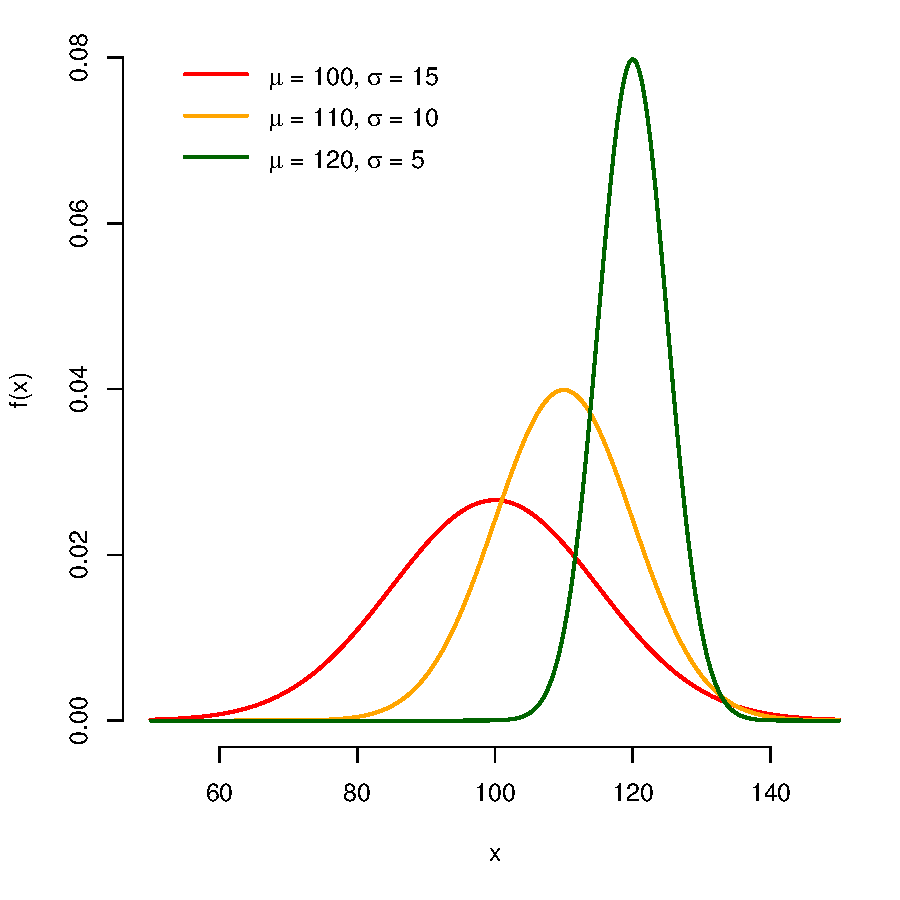
\includegraphics[width=.6\linewidth]{img/ukazka-obr02.pdf}
\caption{A figure with a plot, not entirely related to anything. If you copy the figures from anywhere, always refer to the original author, ideally by citation (if possible). In particular, this picture --- and many others, also a lot of surrounding code --- was taken from the example bachelor thesis of MFF, originally created by Martin Mareš and others.}
\label{fig:g}
\end{figure}

\begin{figure}
\centering
\tikzstyle{box}=[rectangle,draw,rounded corners=0.5ex,fill=green!10]
\begin{tikzpicture}[thick,font=\sf\scriptsize]
\node[box,rotate=45] (a) {A test.};
\node[] (b) at (4,0) {Node with no border!};
\node[circle,draw,dashed,fill=yellow!20, text width=6em, align=center] (c) at (0,4) {Ugly yellow node.\\Is this the Sun?};
\node[box, right=1cm of c] (d) {Math: $X=\sqrt{\frac{y}{z}}$};
\draw[->](a) to (b);
\draw[->](a) to[bend left=30] node[midway,sloped,anchor=north] {flow flows} (c);
\draw[->>>,dotted](b) to[bend right=30] (d);
\draw[ultra thick](c) to (d);

\end{tikzpicture}
\caption{An example diagram typeset with TikZ.}
\label{fig:schema}
\end{figure}

\begin{algorithm}
\begin{algorithmic}
\Function{ExecuteWithHighProbability}{$A$}
	\State $r \gets$ a random number between $0$ and $1$
	\State $\varepsilon \gets 0.0000000000000000000000000000000000000042$
	\If{$r\geq\varepsilon$}
		\State execute $A$ \Comment{We discard the return value}
	\Else
		\State print: \texttt{Not today, sorry.}
	\EndIf
\EndFunction
\end{algorithmic}
\caption{Algorithm that executes an action with high probability. Do not care about formal semantics in the pseudocode --- semicolons, types, correct function call parameters and similar nonsense from `realistic' languages can be safely omitted. Instead make sure that the intuition behind (and perhaps some hints about its correctness or various corner cases) can be seen as easily as possible.}
\label{alg:w}
\end{algorithm}

\section{Extra typesetting hints}

Do not overuse text formatting for highlighting various important parts of your sentences. If an idea cannot be communicated without formatting, the sentence probably needs rewriting anyway. Imagine the thesis being read aloud as a podcast --- the storytellers are generally unable to speak in boldface font.

Most importantly, do \underline{not} overuse bold text, which is designed to literally \textbf{shine from the page} to be the first thing that catches the eye of the reader. More precisely, use bold text only for `navigation' elements that need to be seen and located first, such as headings, list item leads, and figure numbers.

Use underline only in dire necessity, such as in the previous paragraph where it was inevitable to ensure that the reader remembers to never typeset boldface text manually again.

Use \emph{emphasis} to highlight the first occurrences of important terms that the reader should notice. The feeling the emphasis produces is, roughly, ``Oh my --- what a nicely slanted word! Surely I expect it be important for the rest of the thesis!''

Finally, never draw a vertical line, not even in a table or around figures, ever. Vertical lines outside of the figures are ugly.

\chapter{Results and discussion}

You should have a separate chapter for presenting your results (generated by the stuff described previously, in our case in \cref{chap:math}). Remember that your work needs to be validated rigorously, and no one will believe you if you just say that `it worked well for you'.

Instead, try some of the following:
\begin{itemize}
\item State a hypothesis and prove it statistically
\item Show plots with measurements that you did to prove your results (e.g. speedup). Use either \texttt{R} and \texttt{ggplot}, or Python with \texttt{matplotlib} to generate the plots.\footnote{Honestly, the plots from \texttt{ggplot} look \underline{much} better.} Save them as PDF to avoid printing pixels (as in \cref{fig:f}).
\item Compare with other similar software/theses/authors/results, if possible
\item Show example source code (e.g. for demonstrating how easily your results can be used)
\item Include a `toy problem' for demonstrating the basic functionality of your approach and detail all important properties and results on that
\item Include clear pictures of `inputs' and `outputs' of all your algorithms, if applicable
\end{itemize}

\begin{figure}
\centering
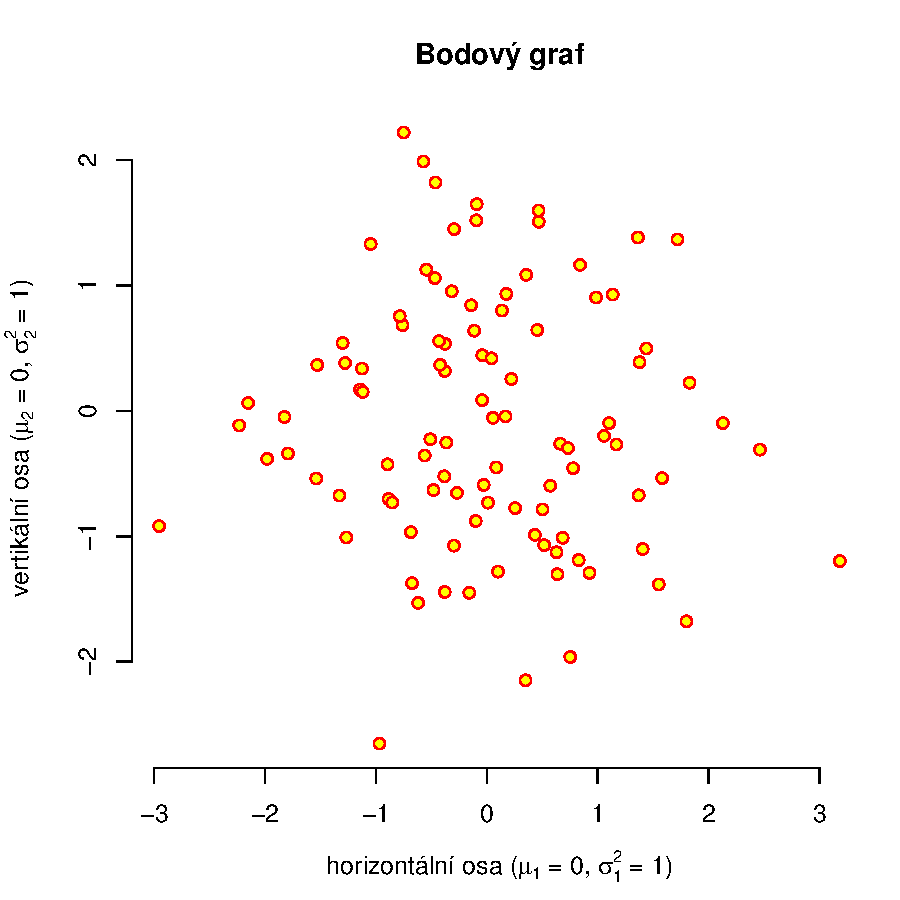
\includegraphics[width=.6\linewidth]{img/ukazka-obr01.pdf}
\caption{This caption is a friendly reminder to never insert figures ``in text,'' without a floating environment, unless explicitly needed for maintaining the text flow (e.g., the figure is small and developing with the text, like some of the centered equations, as in \cref{thm:y}). All figures \emph{must} be referenced by number from the text (so that the reader can find them when he reads the text) and properly captioned (so that the reader can interpret the figure even if he looks at it before reading the text --- reviewers love to do that).}
\label{fig:f}
\end{figure}

It is sometimes convenient (even recommended by some journals, including Cell) to name the results sub-sections so that they state what exactly has been achieved. Examples follow.

\section{SuperProgram is faster than OldAlgorithm}
\subsection{Scalability estimation}
\subsection{Precision of the results}
\section{Weird theorem is proven by induction}
\section{Amount of code reduced by CodeRedTool}
\subsection{Example}
\subsection{Performance on real codebases}
\section{\sloppy NeuroticHelper improves neural network learning}

\section{Graphics and figure quality}

No matter how great the text content of your thesis is, the pictures will always catch the attention first. This creates the very important first impression of the thesis contents and general quality. Crucially, that also decides whether the thesis is later read with joy, or carefully examined with suspicion.

Preparing your thesis in a way such that this first impression gets communicated smoothly and precisely helps both the reviewer and you: the reviewer will not have a hard time understanding what exactly you wanted to convey, and you will get a better grade.

Making the graphics `work for you' involves doing some extra work that is often unexpected. At the same time, you will need to fit into graphics quality constraints and guidelines that are rarely understood before you actually see a bad example. As a rule of thumb, you should allocate at least the same amount of time and effort for making the figures look good as you would for writing, editing and correcting the same page area of paragraph text.

\subsection{Visualize all important ideas}
The set of figures in your thesis should be comprehensive and complete. For all important ideas, constructions, complicated setups and results there should be a visualization that the reader can refer to in case the text does not paint the `mental image' sufficiently well. At the bare minimum, you should have at least 3 figures (roughly corresponding to the 3 chapters) that clearly and unambiguously show:
\begin{enumerate}
\item the context of the problem you are solving, optionally with e.g.~question marks and exclamation marks placed to highlight the problems and research questions
\item the overall architecture of your solution (usually as a diagram with arrows, such as in \cref{fig:schema}, ideally with tiny toy examples of the inputs and outputs of each box),
\item the advancement or the distinctive property of your solution, usually in a benchmark plot, or as a clear demonstration and comparison of your results.
\end{enumerate}

\subsection{Make the figures comprehensible}
The figures should be easily comprehensible. Surprisingly, that requires you to follow some common ``standards'' in figure design and processing. People are often used to a certain form of the visualizations, and (unless you have a very good reason) deviating from the standard is going to make the comprehension much more complicated. The common standards include the following:
\begin{itemize}
  \item caption everything correctly, place the caption at an expectable position
  \item systematically label the plots with `main' titles (usually in boldface, above the plot), plot axes, axis units and ticks, and legends
  \item lay out the diagrams systematically, ideally follow a structure of a bottom-up tree, a left-to-right pipeline, a top-down layered architecture, or a center-to-borders mindmap
  \item {use colors that convey the required information correctly \par\footnotesize Although many people carry some intuition for color use, achieving a really correct utilization of colors is often very hard without previous experience in color science and typesetting. Always remember that everyone perceives color hues differently, therefore the best distinction between the colors is done by varying lightness of the graphics elements (i.e., separating the data by dark vs.~light) rather than by using hues (i.e., forcing people to guess which one of salmon and olive colors means ``better''). Almost 10\% of the population have their vision impaired by some form of color vision deficiency, most frequently by deuteranomaly that prevents interpretation of even the most `obvious' hue differences, such as green vs.~red. Finally, printed colors look surprisingly different from the on-screen colors. You can prevent much of these problems by using standardized palettes and well-tested color gradients, such as the ones from ColorBrewer\footnote{\url{https://colorbrewer2.org}} and ViridisLite\footnote{\url{https://sjmgarnier.github.io/viridisLite/}}. Check if your pictures still look good if converted to greyscale, and use a color deficiency simulator to check how the colors are perceived with deuteranomaly.}
\end{itemize}

Avoid large areas of over-saturated and dark colors:
\begin{itemize}
  \item under no circumstances use dark backgrounds for any graphical elements, such as diagram boxes and tables --- use very light, slightly desaturated colors instead
  \item avoid using figures that contain lots of dark color (as a common example, heatmaps rendered with the `magma' color palette often look like huge black slabs that are visible even through the paper sheet, thus making a dark smudge on the neighboring page)
  \item increase the brightness of any photos to match the average brightness of the text around the figure
\end{itemize}

Remember to test your figures on other people --- usually, just asking `What do you think the figure should show?' can help you debug many mistakes in your graphics. If they think that the figure says something different than what you planned, then most likely it is your figure what is wrong, not the understanding of others.

Finally, there are many magnificent resources that help you arrange your graphics correctly. The two books by Tufte~\cite{tufte1990envisioning,tufte1983visual} are arguably classics in the area. Additionally, you may find many interesting resources to help you with technical aspects of plotting, such as the \texttt{ggplot}-style `Fundamentals' book by~\citet{wilke2019fundamentals}, and a wonderful manual for the TikZ/PGF graphics system by~\citet{tantau2015tikz} that will help you draw high-quality diagrams (like the one in~\cref{fig:schema}).

\section{What is a discussion?}
After you present the results and show that your contributions work, it is important to \emph{interpret} them, showing what they mean in the wider context of the thesis topic, for the researchers who work in the area, and for the more general public, such as for the users.

Separate discussion sections are therefore common in life sciences where some ambiguity in result interpretation is common, and the carefully developed intuition about the wider context is sometimes the only thing that the authors have. Exact sciences and mathematicians do not need to use the discussion sections as often. Despite of that, it is nice to position your output into the previously existing environment, answering:
\begin{itemize}
\item What is the potential application of the result?
\item Does the result solve a problem that other people encountered?
\item Did the results point to any new (surprising) facts?
\item How (and why) is the approach you chose different from what the others have done previously?
\item Why is the result important for your future work (or work of anyone other)?
\item Can the results be used to replace (and improve) anything that is used currently?
\end{itemize}

If you do not know the answers, you may want to ask the supervisor. Also, do not worry if the discussion section is half-empty or completely pointless; you may remove it completely without much consequence. It is just a bachelor thesis, not a world-saving avenger thesis.

\chapter{Results and discussion}

\ifEN
\chapwithtoc{Bibliography}
\else
\chapwithtoc{Seznam použité literatury}
\fi

\printbibliography[heading=none]


\appendix

% if your attachments are complicated, describe them in a separate appendix
%\include{attachments}

\openright
\end{document}
